% -*- root: ../../DAT2-A423_Project_Report.tex -*-
\section{Using the Graph Theoretical Approach on JPEG images}
\label{sec:graphJPEG}
In section \ref{sec:graphtheory} we took a closer look at the Graph-Theoretic Approach for Steganography. 
The goal of this section is to understand how the technique can be modified to work on JPEG images instead of grey-scale Bitmap images. 
The authors of the method define the following about using the technique on JPEG images\cite{hetzl_2005}:

\begin{itemize}
	\item The samples (i.e. 
	where the data will be embedded) are the coefficients of the DCT operation. 
	\item The DC component must not be used for embedding data, as these are often large numbers and and would result in visible distortion of the image, if those were to be altered.
	\item AC components with a value of 0 must not be used for embedding data. 
	If they were to be used, the Run/Length encoding step would be useless, as there will be very few consecutive zeros in the scan data.
\end{itemize}

The process of encoding a JPEG image can be seen on figure \ref{fig:JPEGprocess}. 
Drawn onto the figure is also the embedding step, which will take place after the quantization process.

\begin{figure}[h!]
	\centering
	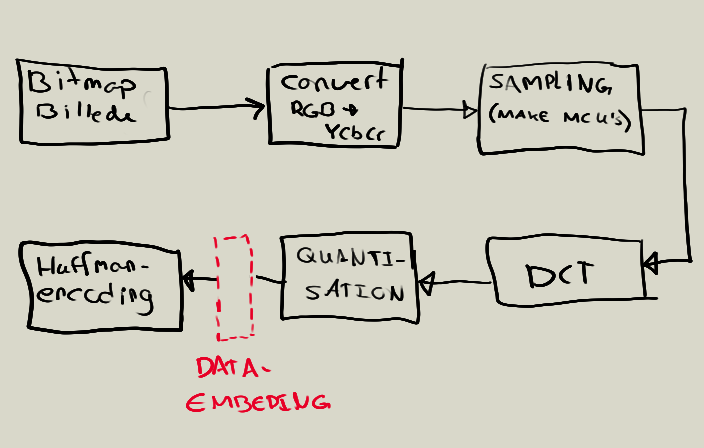
\includegraphics[width=0.95\textwidth]{figures/JPEGprocess.png}
	\caption{caption}
	\label{fig:JPEGprocess}
\end{figure}

There are two ways to go about encoding the message in the quantization coefficients. 
We could either create a graph for each 8x8 matrix of coefficients, or we combine all of the non-zero AC-coefficients into an array and use these values to embed the message. 
The easy way is obviously to create a graph for each matrix, but this would result in having graphs with a maximum of 31 vertices (2 AC values per vertex), and more realistically around 10 vertices (See appendix \textbf{Blablabla}). 
Having few vertices in the graph, means that there are not very many switches that would make the vertices \textit{perfect pairs}, and we will have to forcibly alter more values to hide the message.

The more difficult way of encoding the data is to combine all valid (AC and non-zero) quantization coefficients into a list, and use this list for embedding the data. 
This means that we will not work on the individual 8x8 matrix, but instead on the values from all 8x8 matrices. 
This allows us to obtain a much larger graph, with more edges, and more possible switches of values in the vertices. 
A downside of using this method is, that we cannot do the encoding of the message on-the-fly, as we will have to find all valid coefficients, before we can start the encoding process.

Each method has its pros and cons, but ultimately we have chosen to go with the latter, as the first method limits the graph in such a way that it becomes close to just using LSB, as we will have very few switches, and a lot of forced changes.

Now that we have chosen the dataset in which we will encode the data, we must find a way to get the data. 
Procedure \ref{algJPEG} shows how to obtain the values, after the quantization process. 
The procedure itself is $\mathcal{O}(n)$ where $n$ is the number of quantized matrices from the DCT step. 
With a sampling of 4:2:0 in the JPEG image we have 6 of these matrices in each 16x16 pixel MCU in the image. 
So the number of quantized matrices can be calculated as seen in equation \ref{eq:numOfQuantizedMatrices} where $W$ and $H$ is the width and height of the image, respectively.

\begin{equation}
\label{eq:numOfQuantizedMatrices}
\left \lfloor \frac{W + 15}{16}\right \rfloor \cdot \left \lfloor \frac{H + 15}{16}\right \rfloor \cdot 6
\end{equation}

\begin{algorithm}
\caption{Finding valid entries from the quantized values}
\label{algJPEG}
\begin{algorithmic}
\REQUIRE Quantized 8x8 Matrices $Q = \{ M_1, M_2, M_3 \ldots M_n \}$ ,
\ENSURE List $v$ with all coefficients available for hiding data in
\STATE {$v$} is an empty list
\FOR {$i:=1$ \TO $i=n$}
	\FOR {$j:=1$ \TO $j=8$}
		\FOR {$l:=1$ \TO $l = 8$}
			\IF {$\neg(j = 1 \wedge l = 1)\wedge ((m_i)_{jl} \neq 0)$}
				\STATE{Add $(m_i)_{jl}$ to $v$}

				\COMMENT{Adds all valid coefficients to $v$}
			\ENDIF
		\ENDFOR
	\ENDFOR
\ENDFOR

\RETURN $v$
\end{algorithmic}
\end{algorithm}

After finding the data in which we hide our message, we can encode the actual message as seen in procedure \ref{algJPEGEncode}. 
After this procedure we have a list of the valid coefficients with adjusted values, such that they contain the message. 
To save this to the file, we must first reverse the process of procedure \ref{algJPEG} to replace the values in the quantized values, so that when they are saved to a file, they contain the same values as we have calculated. 
This process would work for all data, but there is still one problem, when decoding the data, we wont know where to stop, also the decoder doesn't know what $m$ value that was used while embedding the data. 
Lets tackle the problem about length first. 
One often used technique is to have a certain marker to look for, and when that marker is encountered, the end of the data has been reached. 
This exact method is actually used in JPEG; when reading through the scan data, we keep on reading until we reach the EOF (End of File) marker. 
And when that marker is encountered, we have read all of the available scan data. 
But as we want our image to be able to contain arbitrary data, we do not want our implementation to depend on a sequence of bits or bytes, that could be randomly found in the data we are embedding. 
So instead we have to make sure that the decoder knows how much data to read, before it starts to actually read it. 

That's why we have decided to use the first 2 bytes of hidden data to contain information about the rest of the data. 
These bytes must also contain information about what $m$ value is used in the data embedding. 
We have chosen to use 14 bits to indicate the length of the message (in bytes) and the last 2 bits to indicate what $m$ value was used (00 = 2, 01 = 4, 10 = 16). 
This leads to a obvious problem, how do we know how to decode the first two bytes, if the information about the $m$ value is hidden in these bytes? To overcome this problem, we have decided to always embed the first two bytes of information using $m = 4$. 
This means that a minor change to \ref{algJPEGEncode} is needed, such that the first 16 bytes of information is embedded differently than the rest.

\begin{algorithm}
\caption{Encoding data into the image data}
\label{algJPEGEncode}
\begin{algorithmic}
\REQUIRE List $v = {v_1, v_2, v_3, \ldots, v_k}$ with all valid coefficients from the DCT process, message $e = \{ e_1, e_2, e_3, \ldots, e_n \}$ as a bit-string and a $m$ value
\ENSURE $v$ contains message $e$
\STATE {$G = (V, E)$ is an empty graph}
\STATE {$i := 1$}
\STATE {$verticesNeeded := \frac{n}{\log_2{m}}$}
\WHILE {$i < verticesNeeded$}
	\STATE{Make vertex from $v_i$ and $v_{i + 1}$ and add to $G$}
	\STATE{i := i + 2}
\ENDWHILE
	
\FOR {$i := 1$ \TO $i = verticesNeeded$}
	\FOR {$j := 1$ \TO $j = verticesNeeded$}
		\IF {$i = j$}
			\STATE{continue}
		\ENDIF
		\IF {a switch between $V_i$ and $V_j$ is possible such that $(V_{i, 1} + V_{i, 2}) \mod m = $ next $\log_2{m}$ bits from e and $(V_{j, 1} + V_{j, 2}) \mod m = $ next $\log_2{m}$ bits from e}
			\STATE{Add edge between $V_i$ and $V_j$} to $G$.
		\ENDIF
	\ENDFOR
\ENDFOR

\STATE{sort edges in $G$ by weight and remove all edges with high weight}

\WHILE {G has any edges}
	\STATE {Switch the values in the vertices connected by the first edge in the graph}
	\STATE {Remove all edges touching the two vertices from the graph}
\ENDWHILE

\FOR {$i := 1$ \TO $i = verticesNeeded$}
	\IF {$(V_{i, 1} + V_{i, 2}) \mod m \neq $ next $\log_2{m}$ bits from e}
		\STATE {Change values in $V_i$ such that they match the bits}
	\ENDIF
\ENDFOR

\STATE{merge $v$ with the values from the vertices in $G$}

\RETURN $v$
\end{algorithmic}
\end{algorithm}


